% --------------------------------------------------------------------------- %
% Poster for the ECCS 2011 Conference about Elementary Dynamic Networks.      %
% --------------------------------------------------------------------------- %
% Created with Brian Amberg's LaTeX Poster Template. Please refer for the     %
% attached README.md file for the details how to compile with `pdflatex`.     %
% --------------------------------------------------------------------------- %
% $LastChangedDate:: 2011-09-11 10:57:12 +0200 (V, 11 szept. 2011)          $ %
% $LastChangedRevision:: 128                                                $ %
% $LastChangedBy:: rlegendi                                                 $ %
% $Id:: poster.tex 128 2011-09-11 08:57:12Z rlegendi                        $ %
% --------------------------------------------------------------------------- %
\documentclass[a0paper,portrait,final,fontscale=0.302]{baposter}
%\documentclass[portrait,final,a0paper,fontscale=0.407]{baposter}

\usepackage[spanish]{babel}
\usepackage[none]{hyphenat}
%\usepackage[latin1]{inputenc}
\usepackage[utf8]{inputenc}

\usepackage{relsize}		% For \smaller
\usepackage{url}			% For \url
\usepackage{epstopdf}	% Included EPS files automatically converted to PDF to include with pdflatex
\usepackage{enumitem}
\usepackage{caption}
\usepackage{wrapfig}

%%% Global Settings %%%%%%%%%%%%%%%%%%%%%%%%%%%%%%%%%%%%%%%%%%%%%%%%%%%%%%%%%%%

\graphicspath{{figs/}}  % Root directory of the pictures 
\tracingstats=2         % Enabled LaTeX logging with conditionals

%%% Color Definitions %%%%%%%%%%%%%%%%%%%%%%%%%%%%%%%%%%%%%%%%%%%%%%%%%%%%%%%%%

\definecolor{bordercol}{RGB}{40,40,40}
\definecolor{headercol1}{RGB}{186,215,230}
\definecolor{headercol2}{RGB}{80,80,80}
\definecolor{headerfontcol}{RGB}{0,0,0}
\definecolor{boxcolor}{RGB}{186,215,230}

%%%%%%%%%%%%%%%%%%%%%%%%%%%%%%%%%%%%%%%%%%%%%%%%%%%%%%%%%%%%%%%%%%%%%%%%%%%%%%%%
%%% Utility functions %%%%%%%%%%%%%%%%%%%%%%%%%%%%%%%%%%%%%%%%%%%%%%%%%%%%%%%%%%

%%% Save space in lists. Use this after the opening of the list %%%%%%%%%%%%%%%%
\newcommand{\compresslist}{
	\setlength{\itemsep}{1pt}
	\setlength{\parskip}{0pt}
	\setlength{\parsep}{0pt}
}

%%%%%%%%%%%%%%%%%%%%%%%%%%%%%%%%%%%%%%%%%%%%%%%%%%%%%%%%%%%%%%%%%%%%%%%%%%%%%%%
%%% Document Start %%%%%%%%%%%%%%%%%%%%%%%%%%%%%%%%%%%%%%%%%%%%%%%%%%%%%%%%%%%%
%%%%%%%%%%%%%%%%%%%%%%%%%%%%%%%%%%%%%%%%%%%%%%%%%%%%%%%%%%%%%%%%%%%%%%%%%%%%%%%

\begin{document}
\typeout{Poster rendering started}

%%% Setting Background Image %%%%%%%%%%%%%%%%%%%%%%%%%%%%%%%%%%%%%%%%%%%%%%%%%%
\background{
	\begin{tikzpicture}[remember picture,overlay]%
	\draw (current page.north west)+(-2em,2em) node[anchor=north west]
	{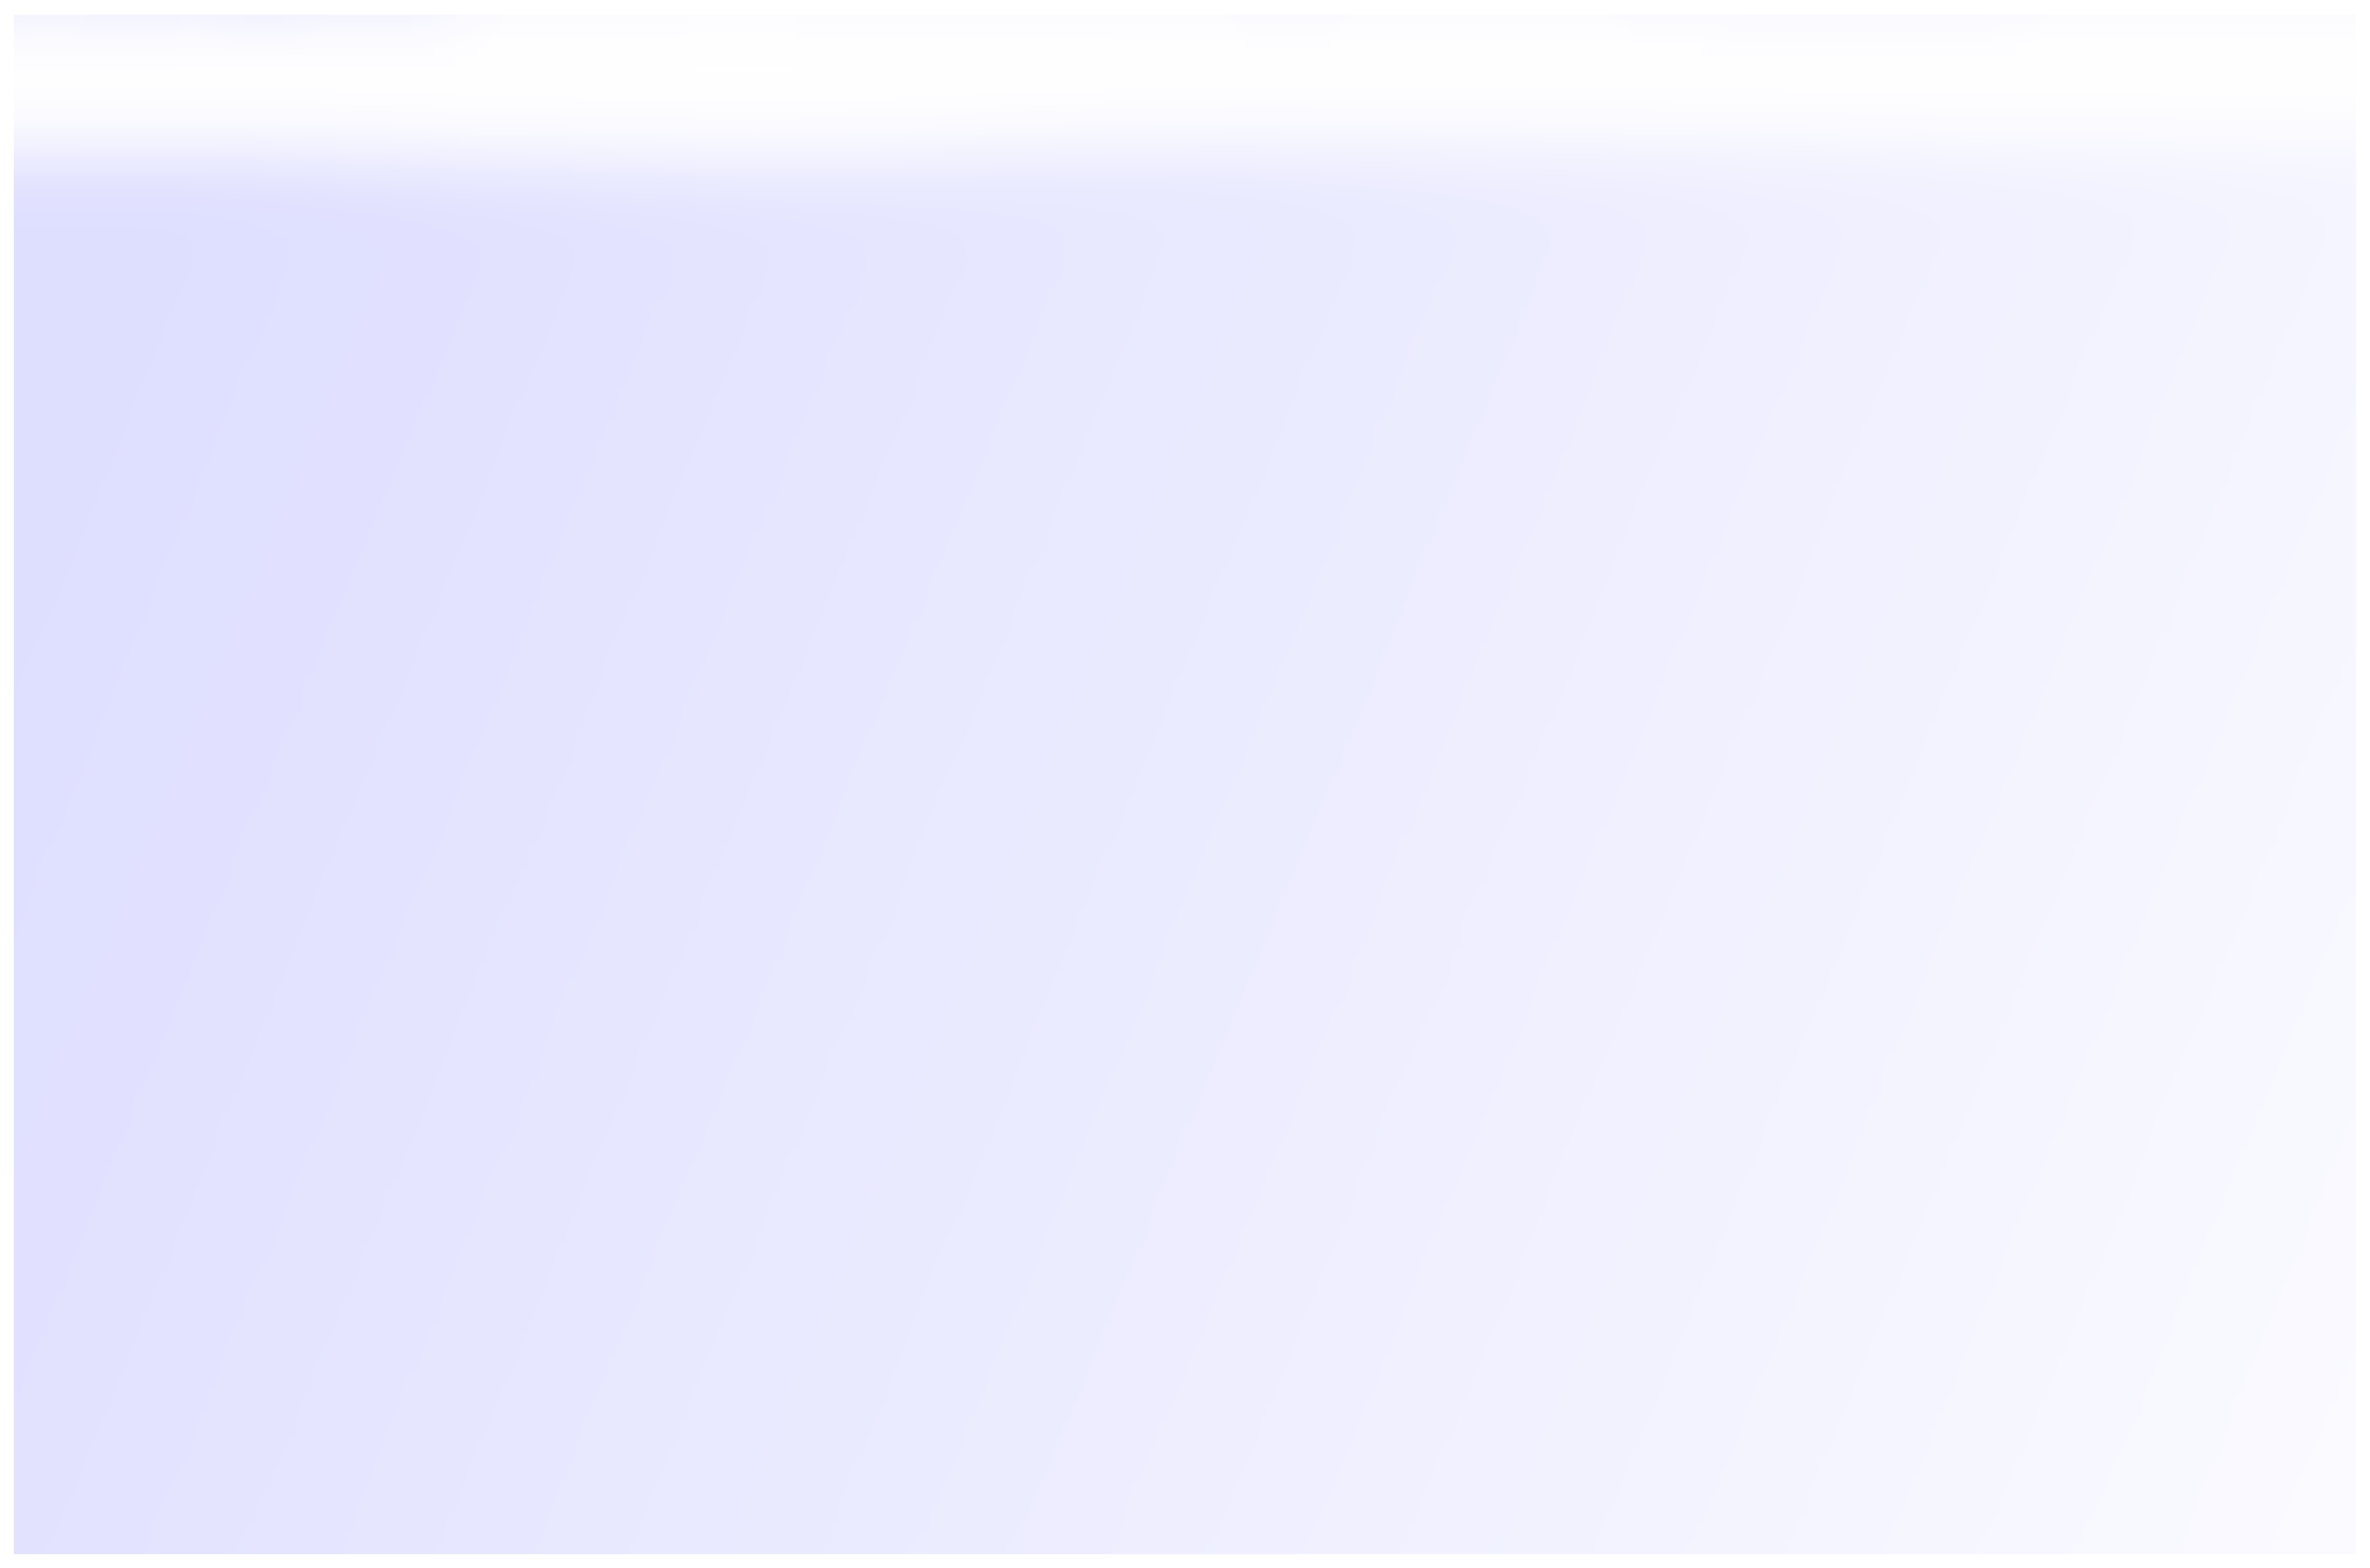
\includegraphics[height=1.1\textheight]{../pix/background}};
	\end{tikzpicture}
}

%%% General Poster Settings %%%%%%%%%%%%%%%%%%%%%%%%%%%%%%%%%%%%%%%%%%%%%%%%%%%
%%%%%% Eye Catcher, Title, Authors and University Images %%%%%%%%%%%%%%%%%%%%%%
\begin{poster}{
	grid=false,
	% Option is left on true though the eyecatcher is not used. The reason is
	% that we have a bit nicer looking title and author formatting in the headercol
	% this way
	eyecatcher=true, 
	borderColor=bordercol,
	headerColorOne=headercol1,
	headerColorTwo=headercol2,
	headerFontColor=headerfontcol,
	% Only simple background color used, no shading, so boxColorTwo isn't necessary
	boxColorOne=boxcolor,
	headershape=roundedright,
	headerfont=\Large\sf\bf,
        textborder=rectangle,
	background=user,
	headerborder=open,
        boxshade=plain
}
%%% Eye Cacther %%%%%%%%%%%%%%%%%%%%%%%%%%%%%%%%%%%%%%%%%%%%%%%%%%%%%%%%%%%%%%%
%{
%	Eye Catcher, empty if option eyecatcher=false - unused
%}
{\begin{minipage}{2em}
    \hfill\vspace{1in}
  \end{minipage} } % Empty space, replace with image if desired
%%% Title %%%%%%%%%%%%%%%%%%%%%%%%%%%%%%%%%%%%%%%%%%%%%%%%%%%%%%%%%%%%%%%%%%%%%
{\sf\bf \smaller[1]
  INVOFI 2016: Olimpiada Metropolitana de Física
}
%%% Authors %%%%%%%%%%%%%%%%%%%%%%%%%%%%%%%%%%%%%%%%%%%%%%%%%%%%%%%%%%%%%%%%%%%
{

  {\smaller[1] \vspace{0.1em} P.N. Alcain$^{1,2}$,
    M.B. Farías$^{1,2}$, M.G. Josebachuili, Q.M. Pears
    Stefano$^{1,2}$, R. Lugones$^{1,2}$, S. Schiavinato$^{1}$} \\
  
  {\smaller[3] $^1$ Departamento de Física, FCEyN, UBA} \\ \vspace{-0.2cm}
  {\smaller[3] $^2$ IFIBA, CONICET, Pabellón 1, Ciudad Universitaria, 1428 Buenos Aires, Argentina}\\ \vspace{-0.2cm}
  {\smaller[3] $^3$ Instituto de Tecnologías en Detección y Astropartículas, CONICET-UNSAM-CNEA}\\ \vspace{-0.2cm}
  {\smaller[3] $^4$ Karlsruhe Institute for Technology, Alemania}\\ \vspace{-0.2cm}
}
%%% Logo %%%%%%%%%%%%%%%%%%%%%%%%%%%%%%%%%%%%%%%%%%%%%%%%%%%%%%%%%%%%%%%%%%%%%%
{
% The logos are compressed a bit into a simple box to make them smaller on the result
% (Wasn't able to find any bigger of them.)
  \setlength\fboxsep{0pt}
  \setlength\fboxrule{0.5pt}
  \fbox{
    \begin{minipage}{5.8em}
      
\includegraphics[width=1\textwidth]{../logos/logo-UBA.png} \\
      
\includegraphics[width=1\textwidth]{../logos/logo-CONICET.png}
    \end{minipage}
  }
}


\headerbox{Resumen}{name=resumen,span=3,column=0,row=0}{

  La enseñanza de la ciencia en las escuelas medias, en particular de
  las denominadas ``ciencias duras'', tiene en general un obstáculo
  que pocas veces se puede sortear: el poco interés de los alumnos en
  los distintos temas científicos. Una forma de aportar a la solución
  del problema es a través de la creación de competencias en ciencia
  que incentiven el interés de los estudiantes en distintos temas
  científicos y que acerquen la universidad tanto a los alumnos como a
  sus docentes.  En este trabajo contamos nuestra experiencia
  organizando la Olimpiada Metropolitana de Física, un evento creado y
  gestionado por estudiantes y graduados de la Facultad de Ciencias
  Exactas y Naturales de la UBA, ideado para estudiantes de educación
  media que ya lleva realizadas 10 ediciones consecutiva, y en el que
  participan más de 100 estudiantes de 20 escuelas de la Ciudad de
  Buenos Aires y alrededores.

}



\headerbox{Introducción y objetivos}{name=intro,column=0,below=resumen}{

  Es de público conocimiento lo difícil que resulta motivar el interés
  por asignaturas relacionadas con las ciencias duras. Esto se ve
  reflejado en que año tras año, la matrícula de alumnos que se
  inscribe a carreras afines es reducida. Las causas de estos
  resultados no pueden atribuirse únicamente a las deficiencias de la
  Enseñanza Secundaria Obligatoria. Debemos analizar también el
  compromiso e interacción de la Universidad con ese sector educativo,
  sabiendo que la alfabetización científica de todos los ciudadanos
  constituye un eje de relevancia para el desarrollo del país.

  En este contexto, la Olimpiada Metropolitana de Física busca y
  permite una mayor interacción entre el Departamento de Física de la
  FCEyN-UBA y los estudiantes y docentes de las escuelas
  medias. Algunos de los objetivos que se proponen son:
  
  \begin{itemize}[wide, labelwidth=!, labelindent=0pt]\setlength\itemsep{0em}
  \item Contribuir a la educación de los jóvenes mediante su
    participación en una actividad que demanda preparación y
    permanente superación en los conocimientos de Física, y
    poniéndolos en contacto directo con científicos activos en la
    comunidad, pudiéndose volver tangible su proyección como
    científicos.
  \item Estrechar el vínculo de la universidad con las escuelas
    medias.
  \item Despertar vocaciones científicas y técnicas.
  \item Identificar a los jóvenes que demuestran mayor aptitud,
    talento e interés en el campo de la ciencia y la tecnología para
    orientarlos y apoyarlos en sus estudios, contactándolos
    directamente con el ambiente universitario.
  \item Promover una visión integradora de las temáticas abordadas por
    la física, procurando que la prueba de la competencia incluya
    problemas que no sean de temas específicos, sino una combinación
    de varios temas del temario propuesto.
  \item Colaborar con la tarea de los docentes, proveyéndolos de
    ejercicios desafiantes e integradores que pueden proponer en el
    aula.
  \item El objetivo más ambicioso y a más largo plazo, es el de
    promover e impulsar Vocaciones Científicas en un colectivo de
    alumnos motivado para ello. Para ello se busca mostrar las
    actividades y líneas de trabajo de los científicos mediante
    charlas y actividades experimentales durante la jornada.
  \end{itemize}
}


\headerbox{Agradecimientos}{name=agradecimientos,column=0,below=intro}{

  Agradecemos al Departamento de Física, FCEyN-UBA, por aportarnos la
  infraestructura que nos permite realizar año a año esta actividad, y
  a la Asociación Argentina de Física y al programa INVOFI por
  otorgarnos el subsidio que nos permitió mejorar dráscticamente la
  actividad.

}







%%%%%%%%%%%%%%%%%%%%%%%%%%%%%%%%%%%%%%%%%%%%%%%%%%%%%%%%%%%%%%%%%%%%%%%%%%%%%%%%%%%%%%%%%%%%%%%%%%%%


\headerbox{La OMF desde adentro}{name=omfdesdeadentro,span=2,column=1,below=resumen}{

  La Olimpiada Metropolitana de Física consiste en una única jornada
  en el mes de septiembre. Durante la mañana los estudiantes resuelven
  la prueba escrita, mientras los docentes se reúnen con los
  organizadores para conversar acerca de la prueba y de las
  dificultades de la enseñanza de física en las escuelas.

  Posteriormente, luego del almuerzo, los docentes y los estudiantes
  participan de disertaciones (charlas) brindadas por científicos
  activos que cuentan sobre sus temas de investigación así como
  visitas a laboratorios, y se complementa con experimentos
  demostrativos sobre distintos temas de física. Mientras tanto, los
  colaboradores realizan la corrección de las pruebas. Para finalizar
  con la actividad, se realiza la entrega de premios.

  \vspace{-0.2cm}
  \subsection*{Preparación del evento} \vspace{-0.2cm}
  La organización del evento comienza varios meses antes. En el mes de
  mayo se envía a las escuelas la invitación formal a participar. Esta
  invitación no es cerrada, sino que cualquier docente de cualquier
  lugar puede presentar a sus estudiantes. Si bien la mayoría de las
  escuelas son de CABA, participan también escuelas de todo Gran
  Buenos Aires: Merlo, Olivos, Quilmes, Ingeniero Maschwitz, Lomas de
  Zamora, Ituzaingó, etc. Durante el mes de julio se abre la
  inscripción {\it online} de los participantes, hasta la última
  semana de agosto.

  Por otra parte, también en mayo se realiza el llamado a
  colaboradores, quienes participan de manera voluntaria. Si bien año
  a año los colaboradores no son los mismos, todos los años se cuenta
  con alrededor de 15 estudiantes y graduados de la Licenciatura en
  Ciencias Físicas. Durante junio y julio, los colaboradores y los
  organizadores escriben los problemas de la prueba, redactan las
  soluciones y confeccionan el material que será entregado a los
  docentes. Durante el mes de agosto se reúnen todos los ejercicios
  hechos y se imprimen tanto las pruebas como los certificados de
  participación. Finalmente, el día del evento, los colaboradores
  ayudan en la corrección de las pruebas, en la toma del examen y en
  la entrega de premios.

  La olimpiada se suele realizar las primeras semanas de
  septiembre. La 10ma OMF se llevó a cabo el martes 6 de septiembre de
  2016 en el Aula Magna del Pabellón 1 de Ciudad Universitaria.

  \vspace{-0.2cm}
  \subsection*{Prueba}  \vspace{-0.2cm}
  La prueba consta de dos niveles: inicial (primer y segundo año de
  física) y avanzado. Además, cada nivel consta de dos etapas.
  \begin{itemize}[wide, labelwidth=!, labelindent=0pt]\setlength\itemsep{0em} \vspace{-0.2cm}
  \item \underline{\it Multiple choice}. Está orientado a que contenga
    tanto problemas teóricos como numéricos de rápida resolución que
    permitan hacer un recorrido por los distintos contenidos
    consensuados, de manera integrada y procurando su vinculación con
    temáticas de la vida cotidiana.
  \item \underline{Problema de desarrollo}. Este tipo de problema es
    común a los dos niveles y está orientado a combinar
    conceptualmente distintos contenidos de la Física para poder
    abordad, de una manera simplificada, una problemática global
    real. Por ejemplo, en los últimos años se ha realizado un
    recorrido histórico por distintos métodos de geolocalización, se
    ha modelado un embotellamiento de automóviles y en la edición 2016
    se ha explicado el efecto Doppler cinemáticamente con una fuente
    móvil lanzando bolas. Suelen ser problemas con poca dificultad
    teórica y matemática, lo que permite que cualquier estudiante esté
    en condiciones de resolverlo, pero que toman más tiempo en ser
    resueltos por el tipo de razonamiento que permite que desarrolle
    el alumno.
  \end{itemize}
  
}

\headerbox{Algunos números y conclusiones}{name=numeros,span=2,column=1,below=omfdesdeadentro}{
  \begin{minipage}[t]{0.63\textwidth}
    En el año 2016 se contó con la participación de 130 estudiantes de
    18 escuelas distintas. Si bien se redujo levemente el número de
    participantes respecto del 2015, se observa un crecimiento ya
    asentado mayor al 50\% respecto de años anteriores. Además, se
    observa que ya se cuenta con un número bastante fijo de alrededor de
    20 escuelas participantes.

    Las devoluciones de los docentes han sido en todos los casos muy
    favorables, y esto puede verse reflejado en que la olimpiada ha
    ido creciendo año a año.

    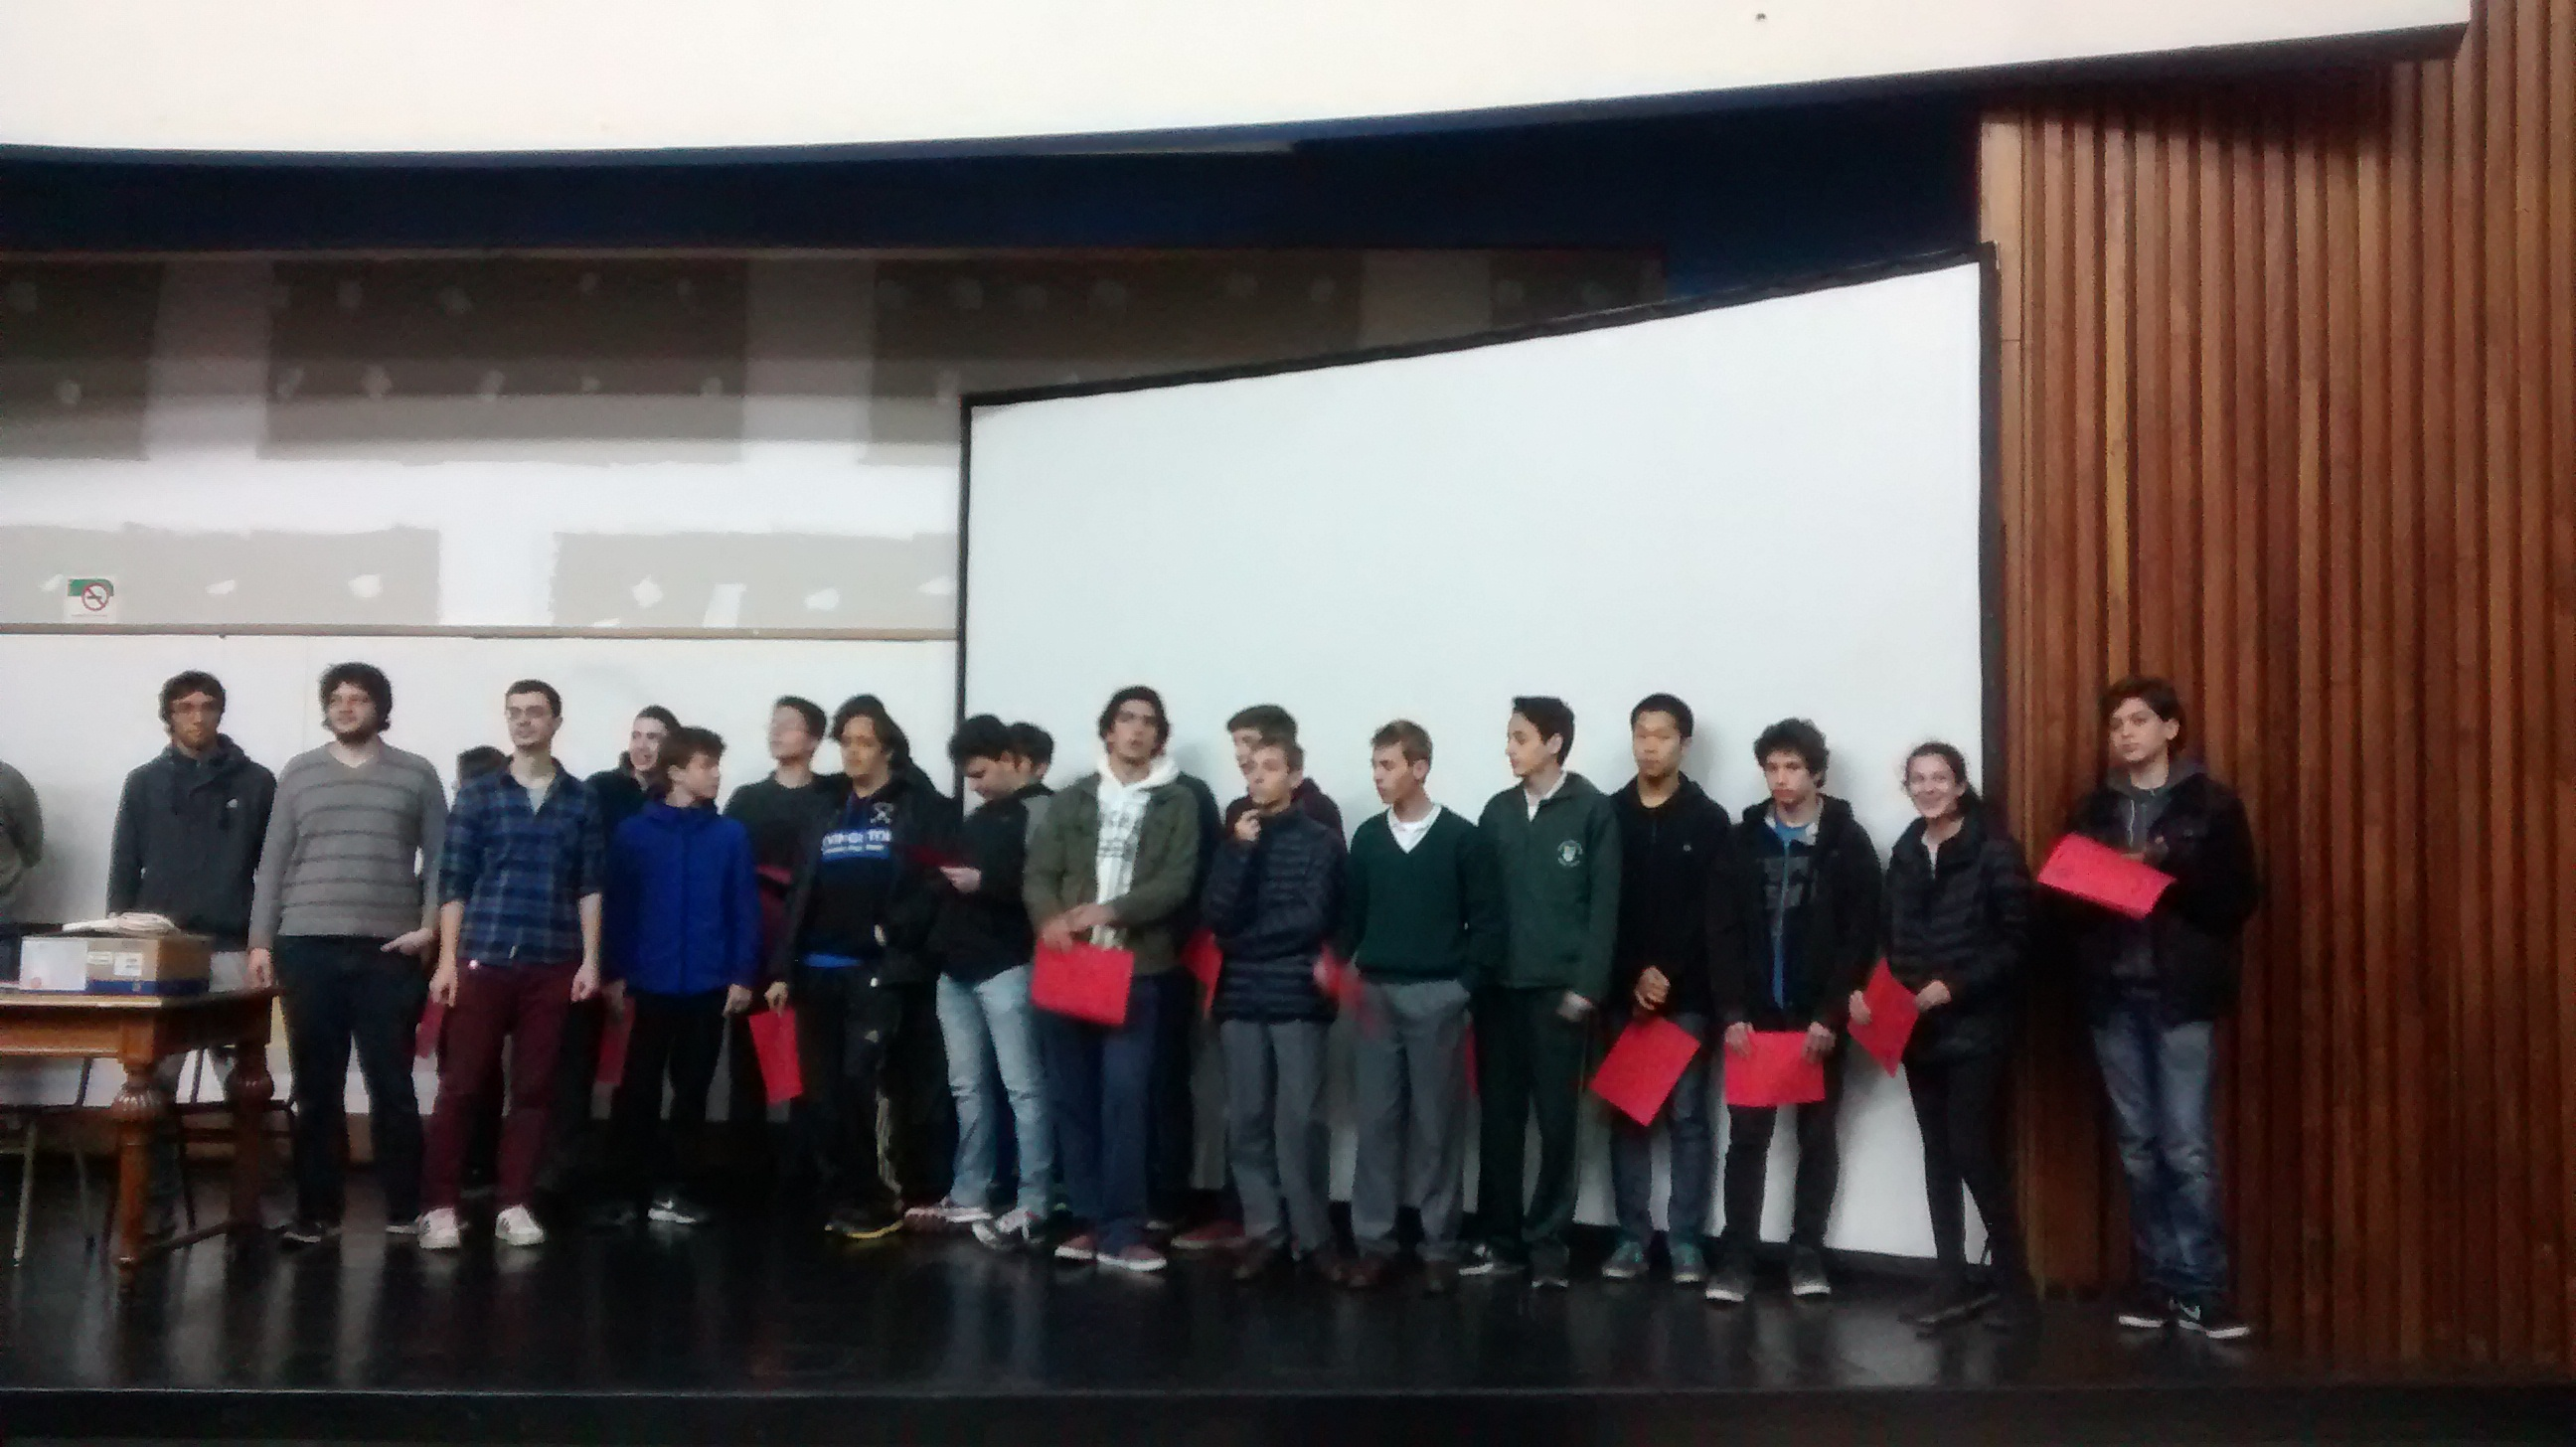
\includegraphics[width=0.33\columnwidth]{Fotos2016_1.jpg}\hfill
    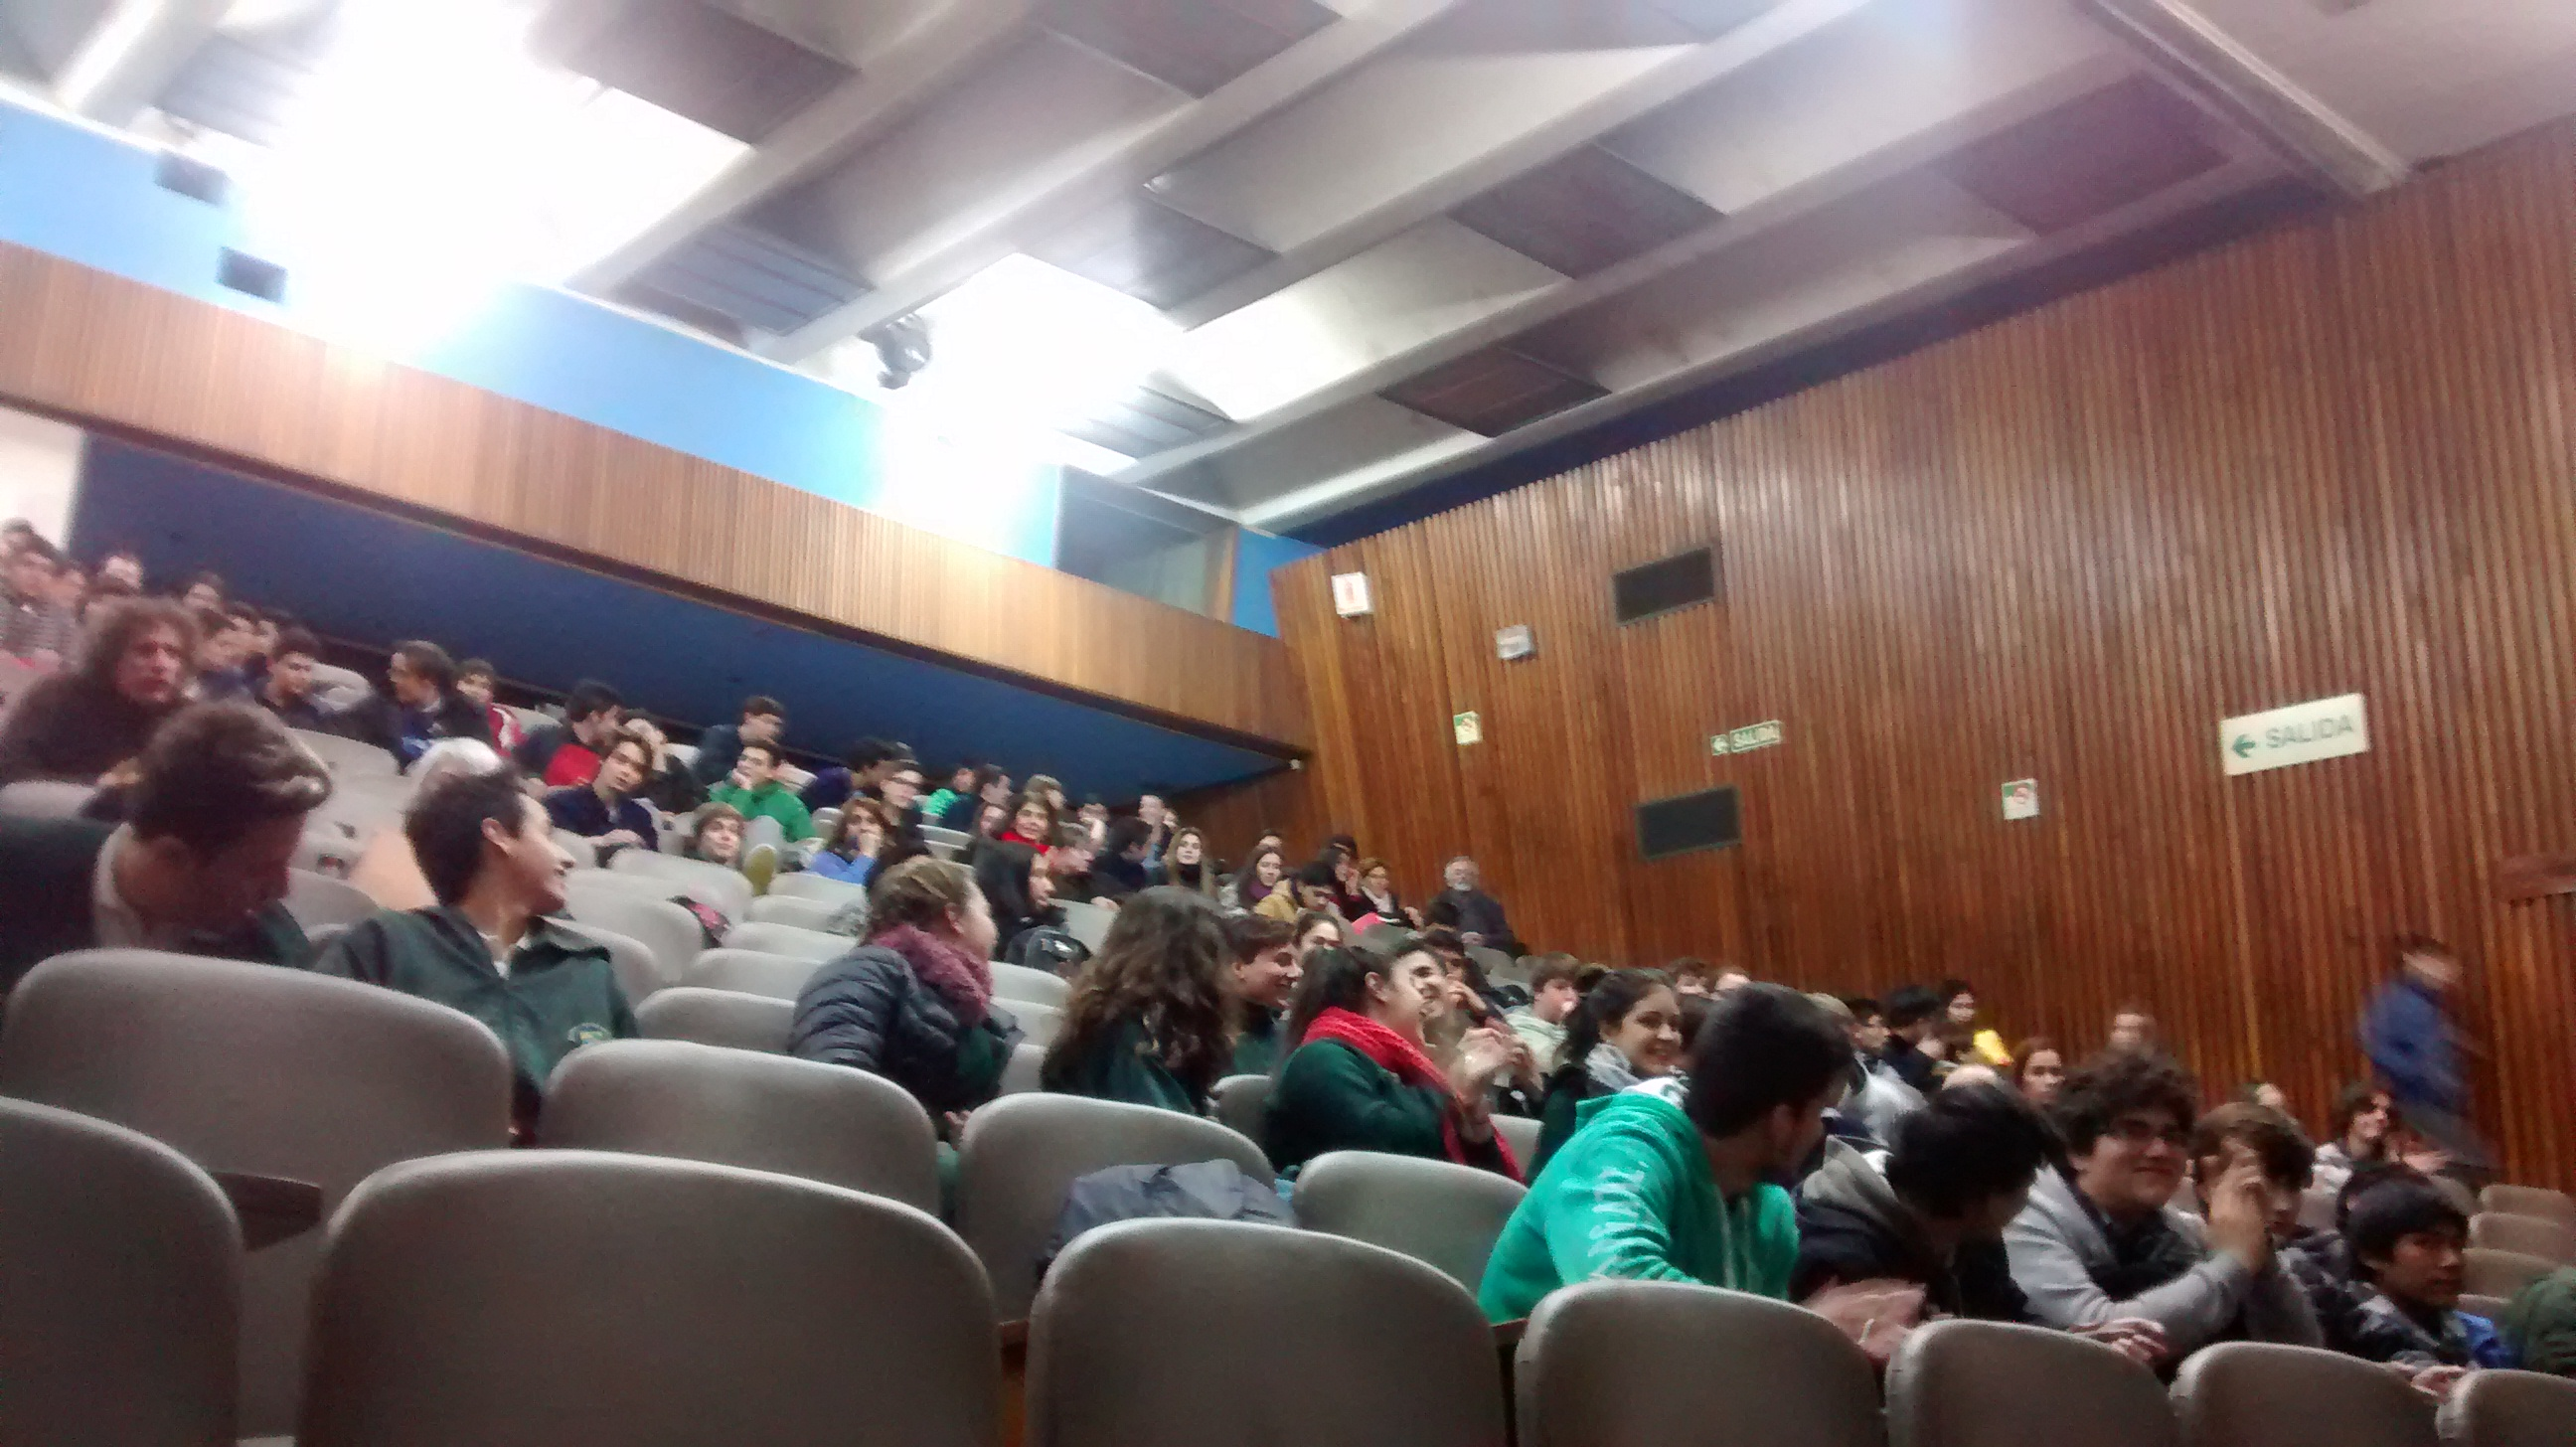
\includegraphics[width=0.33\columnwidth]{Fotos2016_3.jpg}\hfill
    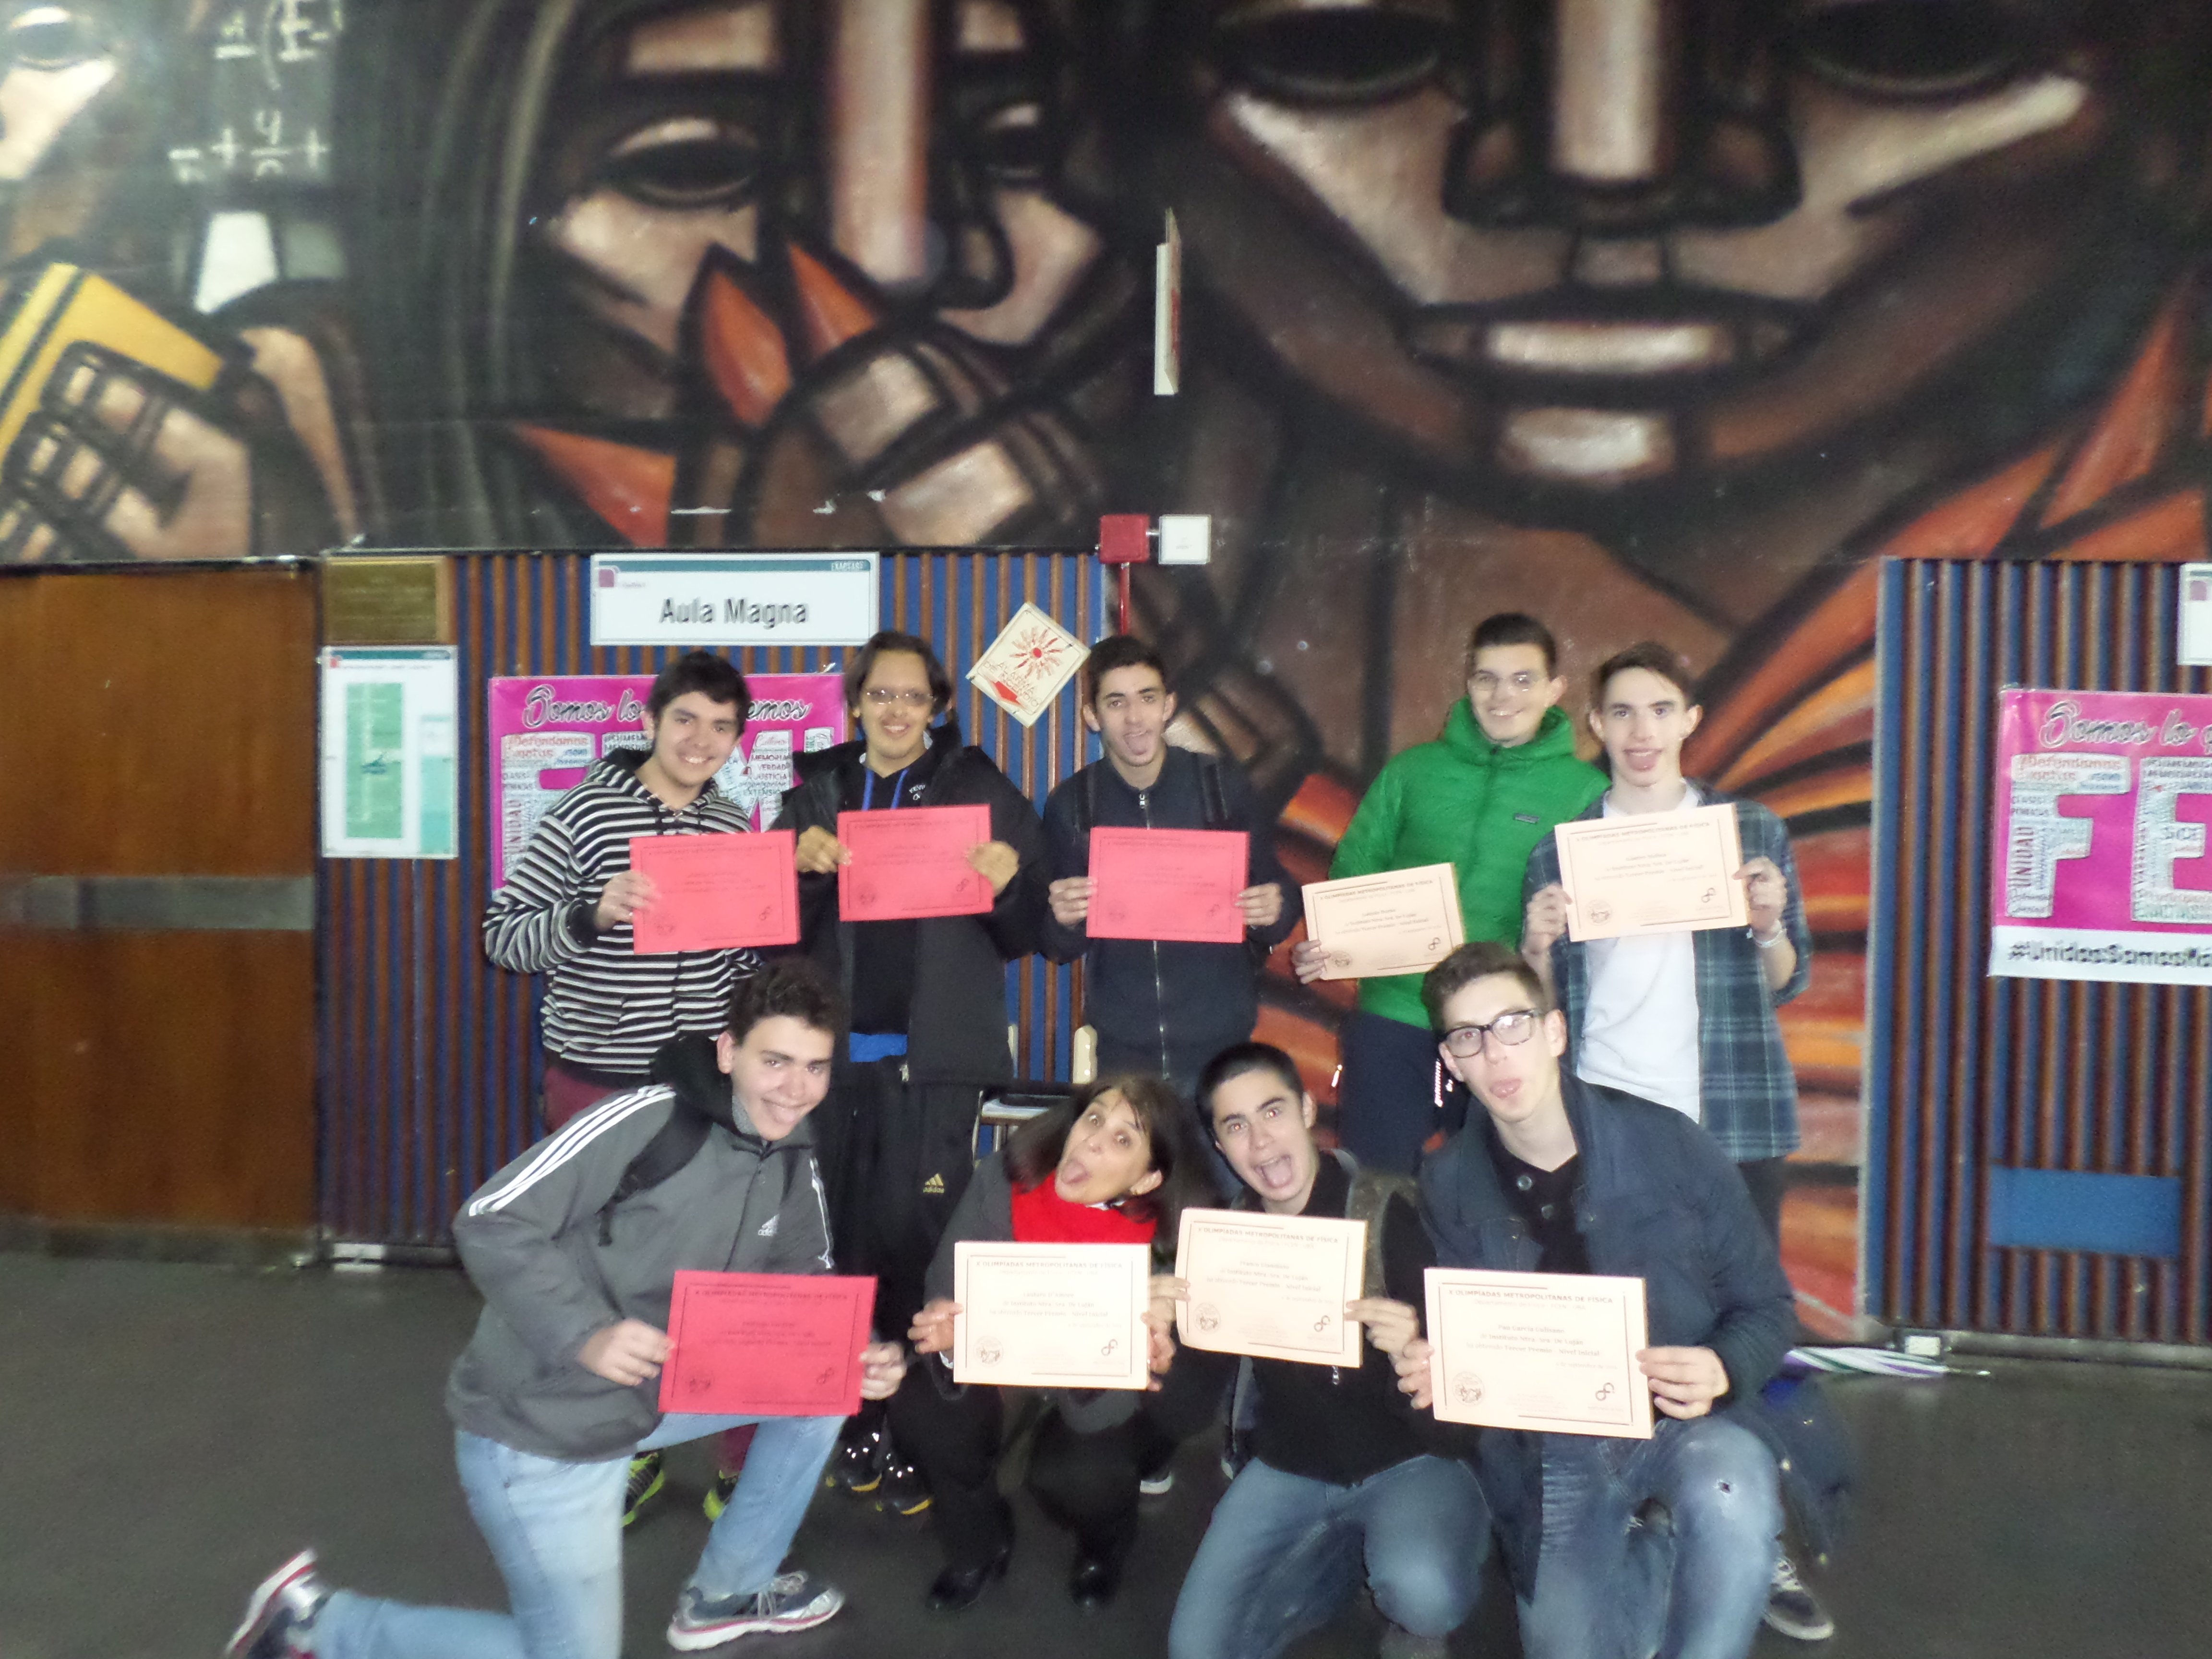
\includegraphics[width=0.33\columnwidth]{Fotos2016_7.jpg}
  \end{minipage}\hfill
  \begin{minipage}[t]{0.33\textwidth}
    \centering
    \raisebox{\dimexpr-\height+\ht\strutbox}{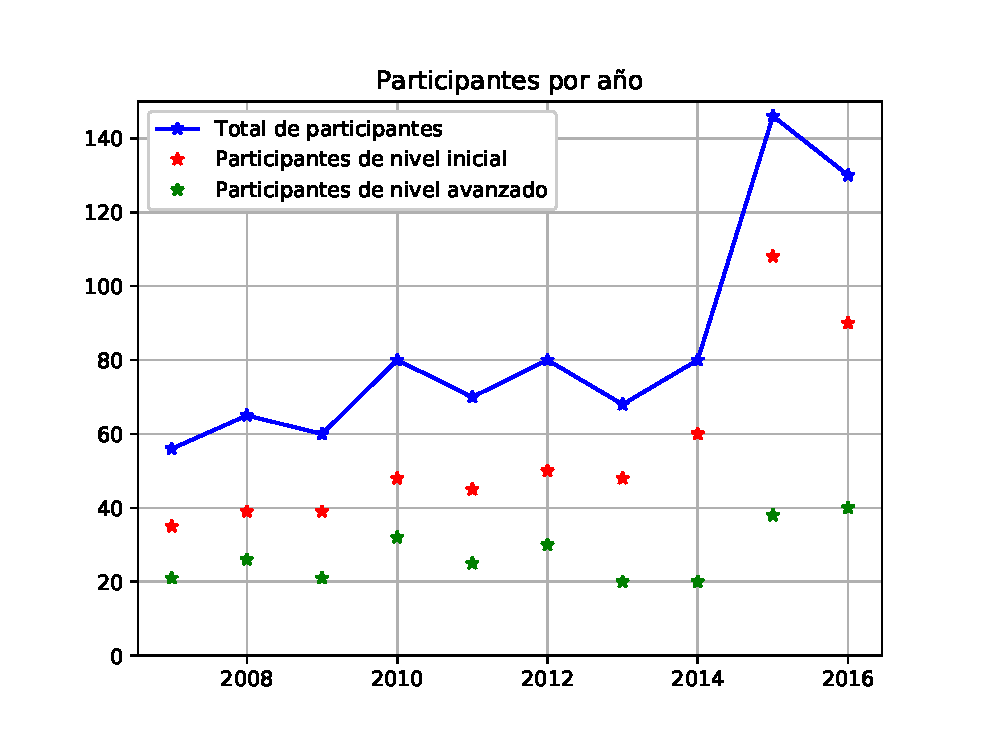
\includegraphics[width=1\columnwidth]{participantes_per_year.eps}\vspace{-0.25cm}}
    \raisebox{\dimexpr-\height+\ht\strutbox}{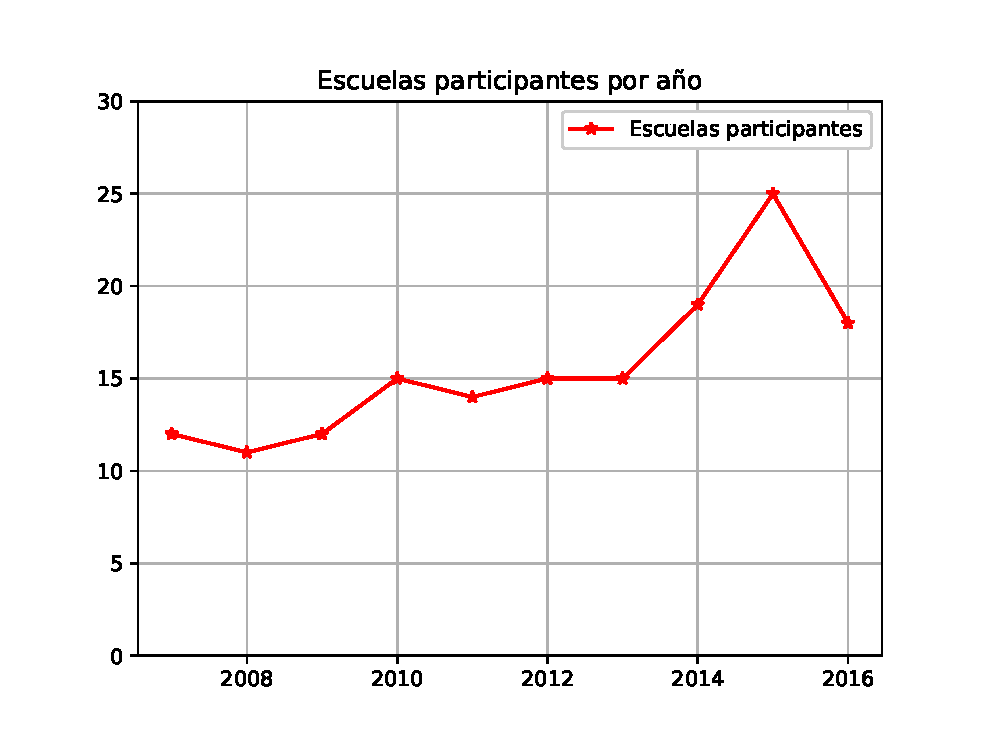
\includegraphics[width=1\columnwidth]{escuelas_per_year.eps}\vspace{-0.25cm}}
  \end{minipage}
  

}





%%%%%%%%%%%%%%%%%%%%%%%%%%%%%







%
\end{poster}
\end{document}
